\documentclass[a4paper,twoside]{report} % for a report (default)

\usepackage{bftn,color} % You need this
\usepackage{verbatim} % for comment

\title{Routing in Barrelfish}   % title of report
\author{Akhilesh Singhania, Alexander Grest}	% author
\tnnumber{006}  % give the number of the tech report
\tnkey{Routing} % Short title, will appear in footer

% \date{Month Year} % Not needed - will be taken from version history

%% \newcommand{\note}[1]{}
\newcommand{\note}[1]{[\textcolor{red}{\textit{#1}}]}

\begin{document}
\maketitle

%
% Include version history first
%
\begin{versionhistory}
\vhEntry{1.0}{09.06.2010}{AS}{Initial version}
\vhEntry{1.01}{14.06.2010}{AS}{Added discussion of design and unresolved issues}
\vhEntry{1.02}{23.07.2010}{AS}{More work on design and API}
\vhEntry{2.0}{31.05.2011}{Alexander Grest}{Multi-hop messaging}
\vhEntry{2.1}{01.12.2013}{TR}{Some explanation}
\end{versionhistory}

% \intro{Abstract}		% Insert abstract here
% \intro{Acknowledgements}	% Uncomment (if needed) for acknowledgements
% \tableofcontents		% Uncomment (if needed) for final draft
% \listoffigures		% Uncomment (if needed) for final draft
% \listoftables			% Uncomment (if needed) for final draft

\chapter{Motivation}

This technical note describes a set of design proposals (and prototype
implementation) of multi-hop message routing in Barrelfish -- how to
send messages between cores which do not have a direct connection
between them.  This arises in, for example, Ethernet communication
with a fully-distributed Barrelfish instance, or between multiple
cores spread out over a PCIe bus (as is the case with Xeon Phi or
Intel SCC). 

All inter-core communication in Barrelfish is performed using explicit
messages, which are carried over ''Interconnect Drivers'' (ICDs),
specialized messaging subsystems that carry data between cores. At
present, all communication happens over direct point-to-point ICD
links. However, there are multiple motivations for extending this. In
this note, we motivate the introduction of a routing layer in
Barrelfish. 


\section{Partial connectivity}
Most current multicore machines are fully connected via shared memory. This means that any core in the system can communicate with any other core in the system
by using shared memory. Most applications are also designed accordingly. However, this assumption is not necessarily true on modern hardware, as the following two examples illustrate:

\begin{itemize}

\item On the \emph{Intel Single Chip Cloud Computer} (SCC), the set of memory a core can access is determined by the setup of its Look Up Tables (LUTs). It is possible that these tables are set-up in such a manner that
two or more cores do not have access to the same region of memory. In such cases to communication these cores will have to route via another set of cores if such a path exists.

\item If Barrelfish is operated on a cluster of machines, there is only an Ethernet-based ICD link between the core(s) where the network stack is running. In order to allow every core to communicate with every other core, the available link must be multiplexed. 

\end{itemize}

This are two examples of current set-ups which lead to partial connectivity. A routing layer akin to the one in IP routing will allow applications to communicate in
such environments, without having to worry about the concrete path a message takes from one core to another. The routing layer will properly route messages in a transparent way.

\section{Resource usage}
ICD links require resources. In particular, a link uses the following resources:

\begin{itemize}
\item \textbf{Memory}: Any ICD link will require some memory to buffer unsent messages and messages that have been received but not yet delivered. Some links will require additional memory for the channel itself. For instance, the shared-memory UMP driver on x86 requires two pages of physical memory per binding. In general, the amount of memory required is governed by the number of messages in flight and
the number of messages in buffer.

\item \textbf{CPU}: Some ICDs, as for example the UMP driver on x86, require explicit polling to check for incoming messages. The more links a core has, the more time it has to spend polling.

\item \textbf{Cache}: If an ICD  uses polling to check for incoming messages, the polled cache line will be placed in the cache. If the core has many ICD links, a significant part of its cache will be flushed due to polling.

\end{itemize}

The more ICD links a core has, the more of its resources will be used for them. This is detrimental to a high-performance system. By limiting the number of links, we will limit the amount of resources required. One way to limit the number of links is to multiplex multiple channels over one ICD link and therefore not construct a fully connected network. 


\section{Heterogeneous IDC}
Barrelfish supports various IDC mechanisms.
Different mechanisms provide different semantics and guarantees such
as maximum frame size, notification mechanism, synchrony, etc.

An application can utilize multiple IDC mechanisms.  This can happen
if a homogeneous machine supports multiple IDC mechanisms or if the
application runs on a heterogeneous machine.  To avoid the need for
the application to understand the different semantics of all IDC, it
can conform to the semantics provided by the routing library.

The semantics provided by the routing layer are discussed in section
\ref{sec:semantics}.

\section{Group communication}

Various parallel computing abstractions such as barriers
require communication among a group of threads.
When any thread enters a barrier, it waits for all other threads to enter
the barrier as well before continuing.

Various distributed communication abstractions such as achieving consensus
also require communication among a group of nodes.
A group of nodes that want to come to agreement on some value
need to communicate with each other.

It has been shown \cite{nishtala:optimizing-collective:hotpar09,
  barrelfish:sosp09} that even in a fully connected 
machine, using some form of routing can improve the performance of group communication.
The sender sends the message to a subset of nodes it wishes to communicate with.
The subset will in turn forward it to the remaining set of nodes.
The work has also shown that the order in which messages are sent also matters.
The optimal route and ordering of messages is machine dependent.

If applications were written with the abstraction of a group layer,
it will allow the library sufficient flexibility in
selecting the optimal route based on the machine type.


\chapter{Multi-hop messaging}

Multi-hop messaging is an important part of the routing layer. It gives applications a possibility to create a logical channel between two cores, that is routed over multiple nodes. This requires that available ICD links are multiplexed.

A multi-hop channel can only be set up between two dispatchers running on different cores. It always leads through the two monitors running on each dispatcher's core. Between those two monitors the multi-hop channel can lead through an arbitrary number of additional monitors. We call all the monitors that lie on a multi-hop channel \emph{nodes}. All the nodes of a multi-hop channel must be connected by means of other ICD-links (such as LMP or UMP ICD-links).

Once a multi-hop channel is set up, it can be used to exchange messages between the two dispatchers. The multi-hop channel transports messages by passing them to the underlying interconnect driver on each link between the nodes of the multi-hop channel. 

The multi-hop interconnect driver consists of
\begin{itemize}
\item A mechanism to set up new multi-hop channels between dispatchers addressed by end-point identifiers
\item A mechanism to send messages along a multi-hop channel
\item A mechanism to receive messages from the channel
\end{itemize}


\section{Design goals}

\subsection{Independence of the underlying interconnect driver}

The multi-hop interconnect driver was designed to be independent of the type of the underlying ICD links between the nodes on the multi-hop channel. This means that it uses the common flounder interface supported by all ICDs when interacting with the underlying ICD link and uses no ICD-specific knowledge. This design involves a performance penalty: Interacting directly with the underlying ICDs instead of via the common flounder-interface would certainly perform better. Nevertheless, we chose this design, as it gives us more flexibility: The multi-hop interconnect channel can run over all present and future interconnect drivers in Barrelfish, as long as they support the common flounder interface.

\subsection{Reliability}

Interconnect drivers in Barrelfish generally provide a reliable messaging service: A message is delivered only once and each message sent is eventually delivered and its content is not corrupted. Furthermore, messages are delivered in FIFO order. The multi-hop interconnect driver is designed to provide a reliable messaging service in principle. However, contrary to the end-to-end argument, it does not provide any \emph{end-to-end} reliability, but builds on the reliability provided by the interconnect drivers of the underlying links. We accept that the multi-hop interconnect driver can fail in case any of the interconnect drivers of the underlying link fail.

\subsection{Resource usage}
Because it is our goal to optimize resource usage, the multi-hop interconnect driver is designed to perform considerably better in terms of resource usage compared to the scenario where we only use direct point-to-point ICD links. In particular, we save memory, because the multi-hop driver has a comparably small memory footprint. 

\section{Design overview}

Messaging in Barrelfish is connection-oriented: messages are passed via an explicit binding object, which encapsulates one half of a connection, and such a binding must be established in advance. Therefore, we have decided to support only connection-oriented multi-hop messaging (for now).  The multi-hop interconnect driver is designed in such a way that channel set-up is collapsed into the binding phase. 

We use virtual circuit switching in order to multiplex multiple multi-hop channels over the available ICD links. Virtual circuit switching has several advantages over a packed-switched approach. It ensures that all messages take the same path and thereby FIFO delivery of messages (as long as the underlying ICD links provide FIFO delivery). Moreover, it allows to create per-circuit state on the nodes of a virtual circuit. 

Each monitor maintains a forwarding table. For each multi-hop channel, entries are created in the forwarding tables at all the nodes of that channel. Messages that are sent over the channel are forwarded at each node according to its forwarding table. Those entries in the forwarding tables can be seen as per-channel created \emph{hard} state: It is explicitly created at channel set-up and deleted at channel tear-down. Additionally to the entries in the forwarding table, per-channel created state includes bindings to the neighbouring nodes on the multi-hop channel.  

In addition to the forwarding table, each node maintains a routing table. The routing table is used for channel set-up: If a node receives a channel set-up request, it determines where to forward the request with the help of its routing table. 

The virtual circuit switching approach would also allow to reserve some resources on the nodes for each channel. Per-channel reserved resources could include buffer space to save received, but not yet forwarded messages, or bandwidth on the ICD links. This is potentially very useful for congestion and flow control. Note that we cannot simply drop messages in case of congested links, as we want to provide a reliable messaging service. As of now, we do not reserve resources on the nodes, but allocate required resources dynamically.

\begin{figure}[h]
	\begin{center}
 	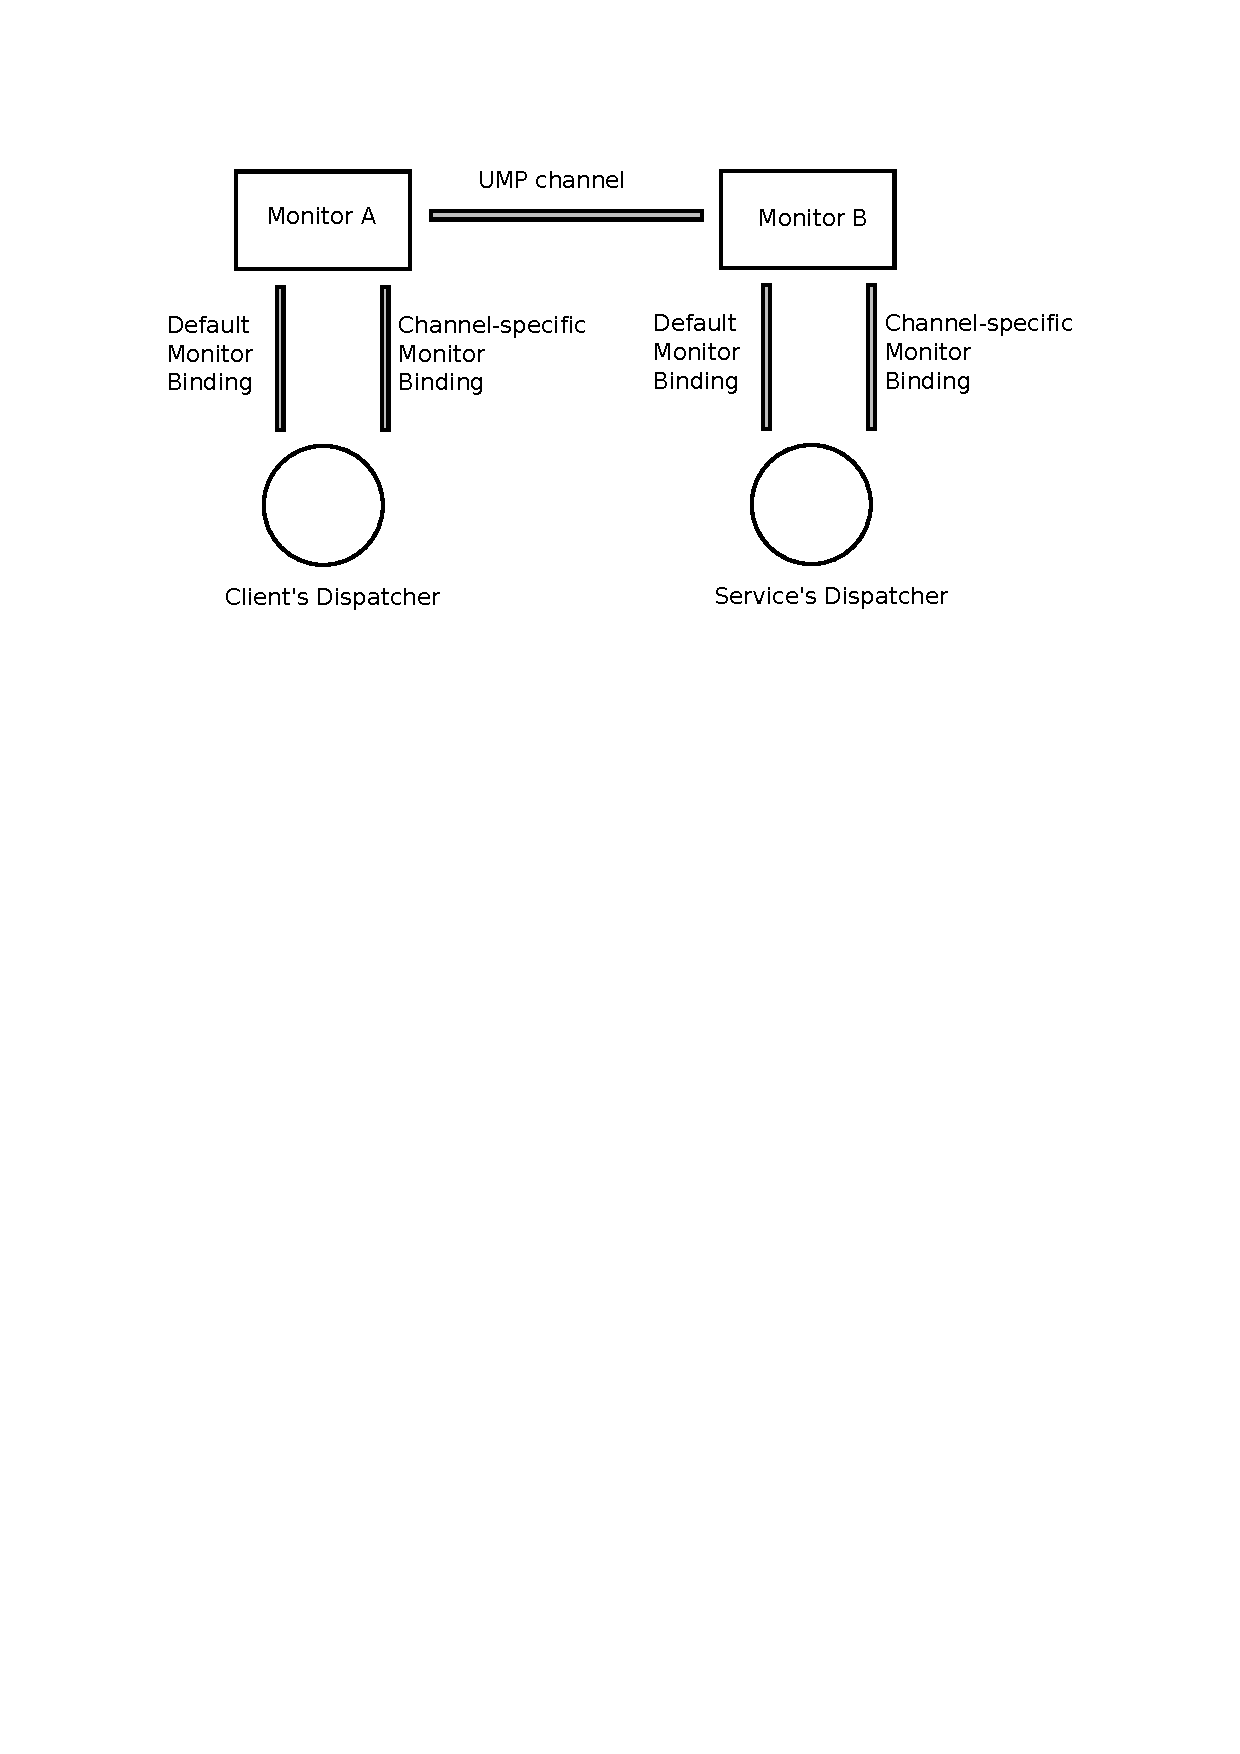
\includegraphics[scale=0.7]{overview_multihop_channel.pdf}
 	\caption{Basic set-up}\label{fig:multihop-chan}
 	\end{center}
\end{figure}

\section{Additional monitor bindings}
A multi-hop channel is multiplexed over the available ICD links. However, for each multi-hop channel, there will be two additional ICD links: Two additional LMP channels will be created between the client's dispatcher and the monitor running on its core and between the service's dispatcher and the monitor on its core. LMP channels are rather cheap - they do not require polling and require only a small amount of memory. Therefore, this does not compromise our goal of optimizing resource usage. Figure~\ref{fig:multihop-chan} shows an example set-up of a multi-hop channel with the two additional LMP channels. 

Those additional channels are needed to ensure that the default monitor binding is not congested or even blocked by multi-hop messages. For example, suppose that a client's dispatcher receives a lot of multi-hop messages within a short period of time. The client reacts to this by allocating more memory. If multi-hop messages are sent over the default monitor binding, the message coming from the memory server will be blocked, therefore this will result in a dead lock. By creating new monitor bindings and not using the default monitor binding, we can prevent such a scenario.


\section{Virtual circuit identifiers}
\label{section:vcis}
Multi-hop messages carry a virtual circuit identifier (VCI). Virtual circuit identifiers allow nodes to identify the particular multi-hop channel a message belongs to. Each node on a multi-hop channel maintains a forwarding table, which maps VCIs to the next hop on that particular channel. A node forwards multi-hop messages based on this forwarding table. At channel end-points, a VCI allows to identify the binding belonging to the multi-hop channel the message was sent over. Virtual circuit identifiers are not only local to a specific link, but also to a direction on that link. Figure~\ref{fig:vci} shows an example assignment of VCIs.

We assign virtual circuit identifiers at random. At each node, we use a hash table to map virtual circuit identifiers to a pointer to the channel state. The use of a hash table allows efficient message forwarding. When a message arrives, it can be determined where to forward this message by means of a simple look-up in the hash table. The complexity of this lookup is linear in the number of virtual circuit identifiers that map to the same hash bucket (the number of buckets in the hash table is a compile time constant).

An attacker sending messages with manipulated virtual circuit identifiers may be able to send messages on channels not belonging to him. By assigning virtual circuit identifiers at random, we make it very unlikely for an attacker to find valid virtual circuit identifiers of channels not belonging to him.

This design requires that each node on a multi-hop channel tells its neighbours what virtual circuit identifier they should use for messages sent over that particular channel. This happens in the set-up phase of a multi-hop channel (see section~\ref{section: set-up}).

\begin{figure}[h]
	\begin{center}
 	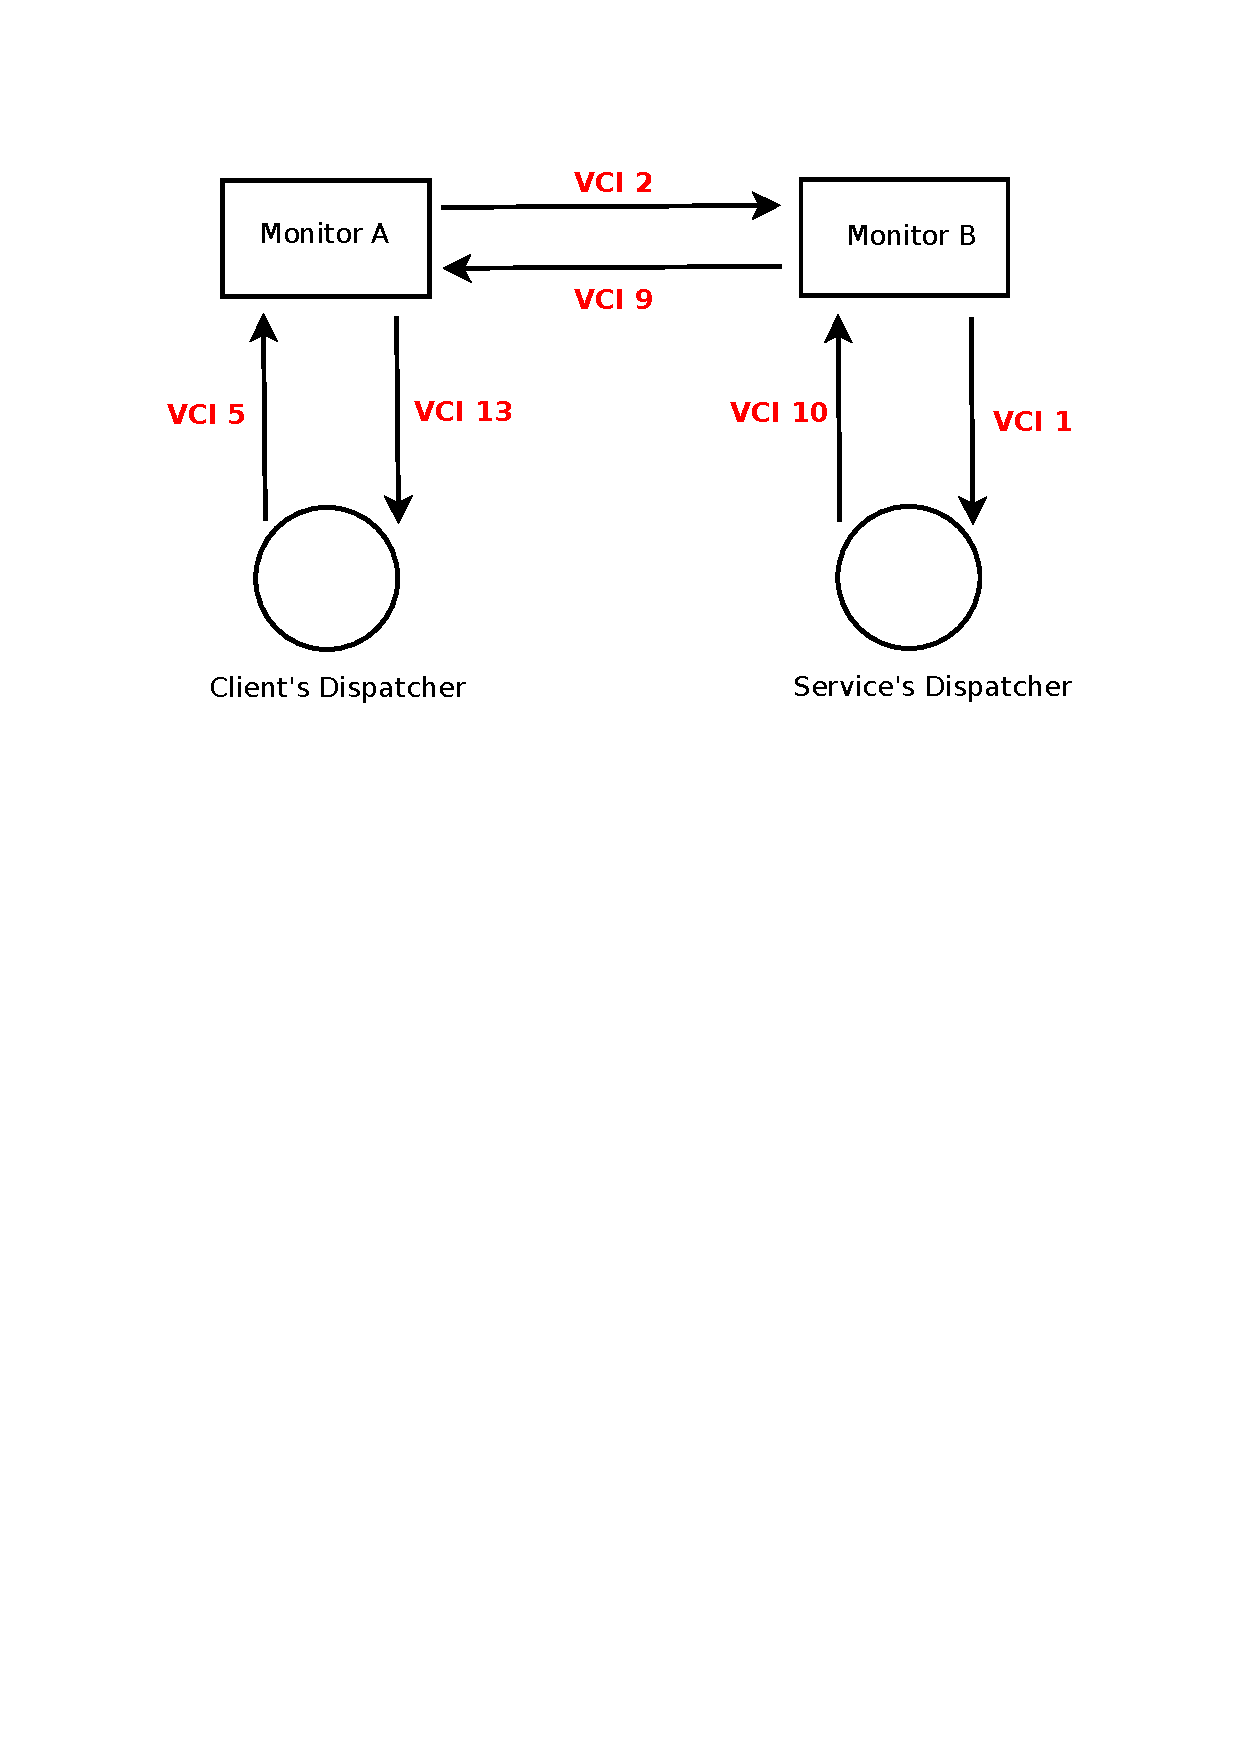
\includegraphics[scale=0.68]{vcis.pdf}
 	\caption{Virtual circuit identifiers} \label{fig:vci}
 	\end{center}
\end{figure}


\section{Channel set-up}
\label{section: set-up}
If two dispatchers want to communicate with the help of the multi-hop interconnect driver, they have to create a multi-hop channel first. During channel-set up, one dispatcher must act as the client and the other as the server (however, once a channel is established, the communication process on both sides of the channel is indistinguishable). 

The channel set-up process can be initiated by invoking the \texttt{multihop\_chan\_bind} function of the multihop interconnect driver. It has to be remarked that normally a user does not interact directly with the multi-hop interconnect driver, but only over the flounder generated stubs (see chapter~\ref{chapter: flounder integration} ).


The channel set-up process works as follows:

\begin{enumerate}

\item A client dispatcher initiates the set-up process by calling the bind function of the multi-hop interconnect driver. This function forwards the bind request to the monitor running on the client dispatcher's core. The bind request includes various parameters, including the \emph{iref} of the service and the client's (ingoing) virtual circuit identifier.

\item The monitor running on the client dispatcher's core determines (from the iref) the core on which the service resides. It then forwards the bind request to another monitor, which is determined based on the routing table.

\item Monitors receiving the bind request check whether the service is running on the same core as they are. If so, they determine the local dispatcher which has exported this iref and forward the request to it. Otherwise, the bind request is forwarded to another monitor in the same way as in step two.

\item As soon as the service's dispatcher receives the bind request, it runs the user provided connection callback. Based on the return value of this callback, it either accepts the connection or rejects it. In any case, the bind reply is sent back to the monitor.

\item The monitor proxies the bind replay back to where it received the bind request from.

\item If the client dispatcher receives the bind reply, it will run the user provided bind callback.

\end{enumerate}

In order to support setting up connections between dispatchers, the existing messaging interfaces between dispatchers and their local monitor, and between monitors has been extended.

As described in section~\ref{section:vcis}, it is necessary that each node on the multi-hop channel tells its neighbouring nodes what virtual circuit identifier they should use for messages sent over that particular channel. Therefore, each message contains the virtual circuit identifier of the sender.  The two response-messages additionally contain the VCI of the receiver. This allows the receiver of a response-message to identify the multi-hop channel the message belongs to.


\section{Message forwarding}
\label{section: message forwarding}
Once the multi-hop channel is set-up, messages can be sent in both directions. A message can be sent by invoking the \texttt{multihop\_send\_message} function of the interconnect driver.  This function requires that the message payload is passed as one (char) array. If a user-defined message contains multiple arguments that are not stored in continuous memory locations, either the user-defined message must be split up in multiple multi-hop messages, or a new array must be allocated and all message arguments must be copied into the newly allocated array (see chapter~\ref{chapter: flounder integration} for a discussion).

In order to support sending messages, the existing messaging interfaces between dispatchers and their local monitor, and between monitors has been extended. Each multi-hop  message contains a VCI, a field encoding the direction of the message and the message payload (as a dynamic array). Furthermore, it contains one field encoding message flags and another field used to acknowledge received messages. Those two fields are used for flow control (see section~\ref{section: flow control}).

As a multi-hop channel allows to send messages in two directions, the direction field is needed to identify the direction of a particular message. Currently we assign direction ''1'' to all messages going from the dispatcher who initiated the multi-hop channel to the other dispatcher, and direction ''2'' for messages going the opposite way. 

This definition of a multi-hop is motivated by the fact that it must be possible to transport an arbitrary message within one (or more) multi-hop messages. By using a dynamic array argument for the message payload, we can transfer data of an arbitrary size in a multi-hop message.

Internally, multi-hop messages are forwarded at every node of a multi-hop channel until they reach the receiver. We make sure that multi-hop messages cannot overtake other multi-hop messages at the nodes by enqueuing messages in the order they arrive and forwarding them in a FIFO order.

\section{Capability forwarding}
\label{section: capabilities}
Because capabilities are maintained as references to per-core state in the CPU drivers, only the LMP interconnect driver which traverses kernel-mode code can directly deliver a capability along with message payload. In the multi-hop interconnect driver, capabilities travel out-of-band from other message payload. 

To send a capability, the monitor sends a \texttt{multihop\_cap\_send} message to its local monitor, containing the capability. The monitor determines whether the capability can be sent to the remote dispatcher. In gereral, capabilities referring to inherently local state (such as LMP endpoint) may not be sent, nor may capabilities that are currently being revoked. If the capability cannot be sent, a \texttt{multihop\_cap\_reply} message is sent back to the local dispatcher containing the error code. Otherwise, the capability is serialised and forwarded along the multi-hop channel. 

The monitor running on the receiver's core reconstructs the capability from its serialised representation and forwards it to the destination dispatcher. This dispatcher identifies the binding to which the capability belongs and invokes a callback on that binding. 

The capability sender only receives a reply message in case an error occurs. An error can occur if for example the capability cannot be sent or the receiver has no space left to accommodate an additional capability.

\section{Receiving messages}
In order to receive messages sent over a multi-hop channel, message handlers must be registered with that multi-hop channel. In particular, three message handlers must be registered: one message handler for ''normal'' messages, one handler for incoming capabilities and one handler for capability reply messages (that are sent in case an error occurred while sending a capability).

The flounder generated stubs for the multi-hop interconnect driver (see chapter~\ref{chapter: flounder integration}) register those message handlers, not the application itself (normally).

\section{Routing tables}
\label{sec: routing tables}
The routing tables are used to determine where to forward a connection set-up request. Each monitor needs its own routing table. We currently support the automatic generation of routing tables for three basic modes of routing:

\begin{enumerate}
\item \textbf{Direct}: All set-up requests are immediately forwarded to the end-receiver.

\item \textbf{Ring}: We route over all cores of a system. Core $i$ forwards a request to core $i+1$ mod num\_cores.

\item \textbf{Fat tree}: We route directly between the cores that are located on the same CPU socket. On each socket, we choose a ''leader'' and route directly between all leaders. A set-up request for a core on a different socket is always forwarded over the local leader to the leader on that socket.
\end{enumerate} 

For the routing modes ''ring'' and ''fat tree'' we need information from the system knowledge base: We need to know the number of cores in the system for the ''ring'' routing mode. For the ''fat tree'' mode, we additionally need to know the number of cores per CPU socket (note that we assume here that sockets are continuously numbered). 

We decided that there should be no direct communication between the monitor and the system knowledge base, because it is not always present. For some architectures, such as Microsoft's experimental Beehive architecture or to a certain extend the Intel Single Chip Cloud Computer, the system knowledge base is not available. Therefore, a dependency of the monitor on the system knowledge base should be avoided.

For this reason, we decided to create a separate module, called the \emph{routing table set-up dispatcher} (RTS) that talks to the system knowledge base and to the initial monitor (the monitor that is first booted). The routing table set-up dispatcher will retrieve the required information from the system knowledge base in order to construct the routing table. Once it has constructed the routing table, it will send it to the initial monitor. 

The initial monitor will forward the (relevant parts of the) routing table to the other monitors once they are booted. This is necessary  because we want to avoid having to create a channel between each monitor and the routing table set-up dispatcher.

It must be noted that the routing table set-up dispatcher can only generate the routing tables for the cores of a single system. It cannot handle set-ups like an Intel single chip cloud computer connected to a x86 machine over a PCIe-based channel.

\section{Flow control}
\label{section: flow control}
It is possible that one dispatcher on a multi-hop channel is sending at a faster rate than the receiving dispatcher can handle incoming messages and process them. Because we want to provide a reliable messaging service, we cannot just drop messages in such a case, but have to buffer them and deliver them eventually. To limit the space needed to buffer undelivered messages, we decided to implement a flow control mechanism within the multi-hop interconnect driver. The flow control mechanism allows the receiving dispatcher to control the transmission speed, so that it is not overwhelmed with messages.

We decided to use a credit-based flow control mechanism: The number of messages in flight at any given time is limited. Once a sender has reached this limit, he has to wait until he receives an acknowledgement that the receiver has processed previously sent messages. We call this limit the \emph{window size}.

The flow control mechanism is completely transparent to applications. It is entirely handled by the multi-hop interconnect driver. On each message sent by a dispatcher over a multi-hop channel an acknowledgement for all messages previously received over this channel is piggy-backed. 

If an application uses a one-way communication schema, i.e. one dispatcher is always sending while the other is only receiving, it is not possible to piggy-back acknowledgements on messages sent the other way. In such a case, the multi-hop interconnect driver sends a dummy message. A dummy message contains no message payload, but acknowledges all received messages. This approach ensures that acknowledgements are, whenever possible, piggy-backed on messages. Only if it is absolutely necessary, an acknowledgement is sent in its own message.



\chapter{Flounder support for multi-hop messaging}
\label{chapter: flounder integration}

Flounder is a stub compiler which generates stubs for defined interfaces. To support multi-hop messaging, we created a new back-end code generator for the flounder stub compiler that generates code to use the multi-hop interconnect driver.  Applications do not interact with the multi-hop interconnect driver directly, but only over the generated stubs. The stubs for the multi-hop interconnect driver have the exact same interface as stubs for other interconnect drivers. This makes application code independent of the interconnect driver used for communication.

The generated stubs can be seen as an ''adaptor'' to the multi-hop interconnect driver. They  translate calls to the common flounder interface to the interface of the multi-hop interconnect driver. Supported functionality mainly includes binding, sending and receiving of multi-hop messages and some control operations.

\section{Binding}
If two dispatchers want to communicate with the help of the multi-hop interconnect driver, they must acquire binding objects for each endpoint of the channel. In any binding attempt, one dispatcher must act as the client and the other as the service (however, once a binding is established, the communication process on both sides of the binding is indistinguishable). The binding phase is merged with channel set-up, i.e. a new multi-hop channel will be created during the binding process. 

In order to initiate a binding, a client dispatcher calls the bind function for a given interface. Because Barrelfish features multiple interconnect drivers, the interface's bind function will have to decide which interconnect driver to use in order to establish the binding. Currently, it ''asks'' the different interconnect drivers to establish a binding in a predefined order (for example, the LMP driver is always first). As soon as an interconnect driver manages to establish the binding, the binding process is finished. Should one interconnect driver fail, the next one in order is tried.

If an application wants to create a new multi-hop channel, it can pass the flag \texttt{IDC\_BIND\_FLAG\_MULTIHOP} as an argument to the interface's bind function. This changes the order of the interconnect drivers: The multi-hop interconnect driver will come in second place, directly after the LMP driver. The LMP driver is first, because it is preferable to the multi-hop interconnect driver if client and service are running on the same core. If the multi-hop interconnect driver fails to establish a binding for some reason, the binding process continues as normal with the other interconnect drivers.

The result of the binding process on the client's and service's side is a binding object which is the abstract interface to the multi-hop interconnect driver for a specific interface type.


\section{Sending messages}
\label{section: flounder sending messages}
A message may be sent on the binding by calling the appropriate transmit function. We distinguish between user-defined messages and multi-hop messages. User-defined messages are those messages defined by the user in the interface. Multi-hop messages are messages that are sent over a multi-hop channel. 

As pointed out in section \ref{section: message forwarding}, the multi-hop interconnect driver requires that the message payload is passed as one char array. If a user-defined message contains dynamic arguments (arguments whose size is only known at run-time), such as a string or a dynamic array, it is generally not possible to pass the message payload as one char array to the multi-hop interconnect driver. There are three possible approaches to send such a message:

\begin{enumerate}
\item Allocate a region of memory capable of holding all message arguments and copy the message arguments to this region. A pointer to it can then be passed to the multi-hop interconnect driver as message payload.

\item Split a user-defined message into multiple multi-hop messages. Each argument of the multi-hop message is transported in its own multi-hop message. 

\item Use a combination of the above approaches. For instance, all fixed size arguments could be sent in one message, and each dynamically sized argument could be sent in an extra multi-hop message.
\end{enumerate}

In comparison to approach 1, approach 2 saves the cost of allocating a region of memory and copying all the arguments of the message to that region. In exchange for that, it needs to split a user-defined message and transport it via multiple multi-hop messages. The preferable approach depends on the type of messages that are sent. However, we think that the performance penalty involved in sending each message argument in its own multi-hop message is not acceptable for most message types. Therefore, the flounder-generated stubs for the multi-hop interconnect driver use approach 1. Approach 3 might be a possible performance optimization, but is currently not in use.

\subsection{Implementation}
All message arguments are copied to continuous memory locations in order to send the whole user-defined message in one multi-hop message.
When sending a user-defined message, we first calculate the size of its payload. The size of a message's payload is only known at compile-time if the message definition does not contain any dynamic arguments. Otherwise, the size of the payload has to be computed each time such a message is sent. After having computed the payload size, we allocate a memory region of that size and copy the message arguments to that region of memory. Finally, we pass a pointer to this memory region to the multi-hop interconnect driver.

We include the size of every dynamically sized argument in the message payload. This tells the receiver about the size of those arguments and allows him to retrieve them from the received message payload. Currently, we use 8 bytes to transfer the size of a dynamic argument. This ensures that we do not get an overflow. We account for those size fields when calculating the size of the message payload.

Capabilities are never sent as message payload. They are always sent out-of-band from ''normal'' message payload. A discussion of this can be found in section~\ref{section: capabilities}.

There is one issue regarding communication in heterogeneous systems of our implementation: To be consistent  with the common flounder interface, we have to use a variable of type \texttt{size\_t} to represent the size of a dynamic array. The type \texttt{size\_t} is architecture dependent. On a 32-bit system it will likely be at least 32-bits wide. On a 64-bit system it will likely be at least 64-bit wide. If a dispatcher on a 64-bit system communicates with a dispatcher on a 32-bit system, this can lead to a problem: The dispatcher on the 64-bit system can potentially send dynamic arrays that are bigger than the dispatcher on the 32-bit system can receive. This is a problem of the current Barrelfish version and remains unsolved.


\subsection{Send continuation}
Each transmit function takes as an argument a pointer to a continuation closure. The closure will be executed after the message has successfully been sent. If another transmit function is called on the same binding before the continuation is executed, it will return the \texttt{FLOUNDER\_ERR\_TX\_BUSY} error code, indicating that the binding is currently unable to accept another message. In this case, the user must arrange to retry the send.

The send continuation is the only way to know when a message has been sent over the multi-hop channel and it is safe to send the next message. Note that even if an application uses a ping pong communication scheme, i.e. it sends a message back and forth between two dispatchers, it is not guaranteed to not get a \texttt{FLOUNDER\_ERR\_TX\_BUSY} error code, unless it serialises all sends with the continuation. This somewhat unintentional behaviour is caused by the fact that the multi-hop channel internally relies on other ICD-links to transport messages. The multi-hop channel itself uses send continuations on the underlying ICD-links to determine when it can accept another message. Those send continuations are always executed after a message is sent. Therefore it is possible (although unlikely) that a message is sent and the reply for that message is received, before the multi-hop channel can accept the next message.


\section{Receiving messages}
The flounder-generated stubs register a callback function with the multi-hop interconnect driver at channel set-up time in order to be notified when a message arrives. As we send a user-defined message within a single multi-hop message, we therefore also receive a user-defined message in one multi-hop message.

Upon receiving a multi-hop message, we have to extract the original user-defined message from it and pass it on to the user-provided receive handler. It is a fatal error if a message arrives on a multi-hop channel and the receive handler function for that message type is not set.

If the user-defined message contains dynamic arguments, we have to allocate space for each of those arguments separately and copy them from the received multi-hop message. This is necessary, because all dynamic message arguments are passed by reference to the user and become property of the user. The user must be able to free those arguments separately, therefore they must be copied to separately allocated memory. Fixed-size arguments are simply passed on the stack to the user.



\chapter{Group Communication}

\section{Terminology}

\textbf{Groups:}
The set of all nodes on the machine form a \emph{universe group}.
The set of nodes in the universe group that
wish to communicate with each other form an \emph{application group}.
An application group is a subset of the universe group.
A subset of nodes in the application group can form a \emph{multicast group}.

It is possible to join and leave any multicast and application group.

\textbf{IDs:}
Each application group is identified by a \emph{group ID}.
The group ID in turn identifies the instance of routing library to use.
The group ID is unique within the universe group.

Each multicast group is identified by \emph{multicast ID}.
The multicast ID is unique within the application group.

When nodes join an application group, they are assigned a \emph{node ID}.
The node ID is unique within the application group.

Each node is also given an \emph{application broadcast ID}.
These may or may not be unique and are drawn from a set that
may just have a single element.

The union of the set of node ID, multicast ID, and application broadcast ID is
called the \emph{destination ID}.
The set of node IDs, multicast IDs, and application broadcast IDs are disjoint.

\textbf{Messaging:}
It is not possible to communicate with nodes in the universe group that
are not in the application group.

A node can send a message to another node in the application group by
sending a message to the appropriate node ID.
A node can send a message to all nodes in the application group by
sending a message to the application broadcast provided to it.
A node can send a message to all nodes in an multicast group by
sending a message to the multicast ID provided to it
when it joined the multicast group.

\textbf{Types of messages:}
\emph{Unicast:} Send a message to a single node in the application group.
\emph{Broadcast:} Send a message to all nodes in the application group.
\emph{Multicast:} Send a message to all nodes in the multicast group.


\section{Semantics}\label{sec:semantics}

The routing layer will provide a uniform set of semantics to the
application layer regardless of the set of semantics the
IDC mechanisms below it provide.
It can provide different semantics to suit the
needs of different application scenarios.

Below, we discuss the different set of semantics it can provide.

\subsection{Set 1: Single source FIFO}
The set of semantics provided are as follows:

\begin{itemize}
\item Reliability:
  A message is delivered only once and only if it was sent earlier.
  Each message is eventually delivered and the contents are not corrupted.
\item Single source FIFO ordering:
  If a sender sends $m$ before $m'$ then $m$ is delivered before $m'$
  at all receivers.
\item Failure:
  The routing library will not fail.
\item Payload:
  The IDC can deliver an arbitrarily sized message.
\end{itemize}

\subsection{Set 2: Causal order}
The set of semantics provided are as follows:

\begin{itemize}
\item Reliability:
  A message is delivered only once and only if it was sent earlier.
  Each message is eventually delivered and the contents are not corrupted.
\item Causal ordering:
  If the delivery of message $m$ depends upon the delivery of message $m'$ as
  per the \emph{happened before} relationship \cite{Lamport:1978:TCO:359545.359563},
  then $m$ is not delivered till $m'$ has been delivered.
\item Failure:
  The routing library will not fail.
\item Payload:
  The IDC can deliver an arbitrarily sized message.
\end{itemize}

\subsection{Set 3: Total order}
The set of semantics provided are as follows:

\begin{itemize}
\item Reliability:
  A message is delivered only once and only if it was sent earlier.
  Each message is eventually delivered and the contents are not corrupted.
\item Total order:
  All messages are delivered to all nodes in the same order.
\item Failure:
  The routing library will not fail.
\item Payload:
  The IDC can deliver an arbitrarily sized message.
\end{itemize}

It is possible to order messages using various types of ordering mechanisms.
Investigation of this remains future work.

\subsection{Additional sets}
In future, if we choose to provide additional set of semantics,
they will be listed here.
They could include weaker semantics than above if the underlying IDC mechanism
are too expensive.
Some example are just reliability, or not even providing reliability.

\section{Interface}
We discuss the interface for group management and sending/receiving of messages.

\subsection{Group management}

\textbf{Creating groups:}
Before nodes can join a group, they need to be created.
Any dispatcher in the system can create a new application group
and any node in an application group can create a new multicast group
within the application group.

The library will return to application a group ID or
multicast ID of the created group.

\textbf{Updating a group:}
A dispatcher can join any application group by calling join on
the application group ID.
A node can join any multicast group within the application group it is part of.
When the join has finished, the node gets the join callback from the library.
When a dispatcher is done joining an application group,
it can query the library for its node ID and application broadcast ID.

Similarly a node can leave a group at anytime by calling leave on the group ID.
When the leave is done, the application will get a leave callback.
A dispatcher should call leave before it exits the system.

The behavior of the group is undefined while membership is in flux.
New links are being created and old links are being torn down.
Messages may not reach their proper destination.
If such guarantees are required at all times in the application,
the application must refrain from sending messages while
group member is in flux.

\section{Flow control}
The IDC mechanisms that the routing library operates over are asynchronous.
When a message is sent over them,
it will eventually be delivered to the receiver.
Undelivered messages are maintained in a queue of fixed length.
If the sender tries to send messages too quickly the queue can fill up.
If the queue is full, the sender must wait
till the queue has room for more messages.
IDC mechanisms allow senders to register callbacks in such situations.
When a send fails with the transient error that
the queue is full, the sender can register
a callback which will be called when the next send should not fail.
While the sender waits for the callback, it has to handle the unsent message.

We discuss the simple scenario of two nodes and
then a more complex scenario of many nodes.

\subsection{Client-server model}

\begin{figure}[t]
 \includegraphics[width=\columnwidth]{client-server.pdf}
 \caption{Client-server model}\label{fig:client-server}
\end{figure}

Figure \ref{fig:client-server} shows a simple client-server model
of two nodes that are directly connected.
The weights on the edges is the length of the queue.
The client sends messages to the server, the server processes them
and sends replies to the client.
It is possible that link1 becomes full maybe because
the client has not been handling replies on it.
At this point the server has some options:%

\begin{itemize}
\item Drop the message.
  The server can simply drop the message if the queue is full.
  This will result in an unreliable channel.
\item Allocate some resources and queue the message up.
  This implies unbounded resource requirement.
\item Apply back pressure on the client.
  The server at this point can stop processing messages
  from the client till it is able to send messages to it again.
\end{itemize}

In this model the last option works well as it will force the client
to slow down and process replies before sending more requests.

\subsection{Multihop route}

\begin{figure}[t]
 \includegraphics[width=\columnwidth]{many-to-many.pdf}
 \caption{Example multihop route}\label{fig:many-to-many}
\end{figure}

In this scenario the problem is more complex.
Figure \ref{fig:many-to-many} shows a group of 5 nodes,
the link weights specifies the queue length of the link.
If node1 and node2 are sending messages to node4,
link34 will fill up before link13 or link23 does.
Node3 cannot send additional messages to node4.
At this point, node3 has the following options:

\begin{itemize}
\item Continue to process incoming messages on link13 and link23.
  If they are destined for node4, drop them.
  This will result in an unreliable channel.
\item Continue to process incoming messages and if they are destined for node4,
  queue them up locally.
  This implies unbounded resource requirement.
\item Stop processing messages on link13 and link23.
  This will delay messages on those links that were not destined to node4.
  In literature, this is called \emph{Head of line blocking} \cite{cite}.
\end{itemize}

None of these solutions are particularly desirable.
Flow control in the context different types of networks has
been studied previously.

Relevant existing work includes:
\begin{itemize}
\item Credit based flow control:
  The endpoints dictate maximum number of messages in flight.
\item TCP flow control
\item Ethernet flow control
\item Datacenter ethernet flow control
\item Related work in routing between sockets on a machine
\item QoS (DiffServ and IntServ).
\end{itemize}

Some applications may not be willing to pay the cost of flow control.
Further, a flow control mechanism that guarantees reliability
may not scale well with  number of nodes.
We discuss some abstract ideas we have for flow control below.

\section{Open questions}
Some open questions

\subsection{Reservation of resources with end-to-end flow control}
The essential idea is that when a route is established,
reservations for some number of in flight messages are made for the route.
Even though the links might be shared,
no other routing path is allowed to use the reserved resources.
The endpoints must then limit the number of in flight messages.
If they exceed it, the library can deliver an error at the endpoint or try to
optimistically deliver the message and drop the message if it is unable to.

For example, in figure \ref{fig:many-to-many},
if reservations for two messages is made for the routing path
from node1 to node4, node1 and node3 each will maintain a queue of size 2.
Whenever they receive a message from the application in node1 destined to node4
and they are not able to send it on the link,
they can locally store the message.
Eventually, when the link has space in it,
they can try to send the message again.

It remains to be seen if the approach can work and scale well.
\note{Cite work on switching networks and other works that make reservations and
  give guarantees.}

This approach works when the nodes that are sharing the links
cooperate with one another.
However, if the link is shared between distrustful
nodes then additional guarantees of fairness and no starvation maybe required.

\begin{figure}[t]
 \includegraphics[width=\columnwidth]{client-monitor.pdf}
 \caption{A network of monitor with clients}\label{fig:client-monitor}
\end{figure}

Figure \ref{fig:client-monitor} shows a network of two monitors.
Each monitor is connected to two clients.
Clients A1 and A2 are cooperating and client B1 and B2 are cooperating.
The clients want to send some messages that must go through the monitors such as
transferring capabilities.
If one pair of client is aggressive in sending messages,
it may fill up the link between the monitors and impact the performance
of the other pair of clients.
In this scenario, the link between the monitor can be seen
as a common system resource that is being multiplexed between the users.
The monitors should guarantee some fairness to the users in using this link.

\subsection{Discovering node IDs}
When a set of dispatchers join an application group,
each of them is assigned a node ID.
The nodes need some mechanism of discovering the IDs of each other
so that they can message each other.

The discovery service will be built on top of the routing library
and can be designed in multiple ways.
Nodes can send broadcasts to each other informing each other of their node IDs,
they can use the name service, etc.

\chapter{Interesting benchmarks}\label{chap:benchmarks}

Some benchmarks that validate the claims of above and show the performance of the library.

\note{Costs of one-to-many channels. One sender, multiple readers.}

\note{Comparison of routes with no forwarding and routes with forwarding.}

\note{Resource requirements for channels, memory and cpu time.}

\note{Cost of the discussion group membership update mechanism.}

\chapter{Fun research questions}

\begin{itemize}
\item Flow control
\item Link state vs. distance vector routing
\end{itemize}

\bibliographystyle{abbrv}
\bibliography{defs,barrelfish}

\end{document}
